\section{VII. Đánh Giá Dự Án}

\begin{frame}
\frametitle{Đánh giá hiệu năng game}
    Cấu hình thiết bị:
    \begin{itemize}
        \item Hệ điều hành: Windows 11 Home Single Language 64-bits
        \item Bộ xử lý: Intel Core 7 150U (10 nhân, 12 luồng, xung nhịp 1.80 GHz)
        \item Bộ nhớ RAM: 16 GB
        \item Card đồ họa: Intel Graphics hỗ trợ DirectX 12
        \item Kiến trúc hệ thống: x64-based PC
        \item Thiết bị: Dell Inspiron 14 5440
    \end{itemize}
\end{frame}

\begin{frame}
\frametitle{Hiệu năng trước khi tối ưu}

    \textbf{Màn hình chính:}
    \begin{itemize}
        \item Draw Calls: ~30
        \item FPS: 70--80
    \end{itemize}

    \textbf{Trong gameplay (3 người chơi):}
    \begin{itemize}
        \item Draw Calls: 800 -- >1300
        \item FPS: 40--50
    \end{itemize}

    \textbf{Vấn đề:}
    \begin{itemize}
        \item Khựng hình, giật lag khi di chuyển và tương tác
        \item CPU overload do quá nhiều Draw Calls
    \end{itemize}
\end{frame}

\begin{frame}
\frametitle{Chiến lược tối ưu hiệu năng}

    \begin{itemize}
        \item \textbf{Static Batching}: Object tĩnh (bàn, tường, nội thất)
        \item \textbf{GPU Instancing}: Thẻ bài, props lặp lại
        \item \textbf{Texture Atlas \& Material Sharing}: Giảm số lượng material
        \item \textbf{UI Optimization}: Chia nhỏ Canvas
        \item \textbf{Networking}: Chỉ sync dữ liệu cần thiết, giảm RPC
    \end{itemize}
\end{frame}


\begin{frame}
\frametitle{Hiệu năng sau khi tối ưu}

    \textbf{Kết quả cải thiện:}
    \begin{itemize}
        \item Draw Calls: \textbf{200--300} (giảm ~70\%)
        \item FPS: \textbf{60--70} (ổn định)
    \end{itemize}

    \textbf{Lợi ích:}
    \begin{itemize}
        \item Không còn tụt FPS đột ngột
        \item Di chuyển \& tương tác mượt mà
        \item Frame time ổn định
        \item CPU usage giảm rõ rệt
    \end{itemize}
\end{frame}

% 2
\begin{frame}
    \frametitle{Chất lượng đồ họa tổng quan:}
    \begin{figure}[H]
        \centering
        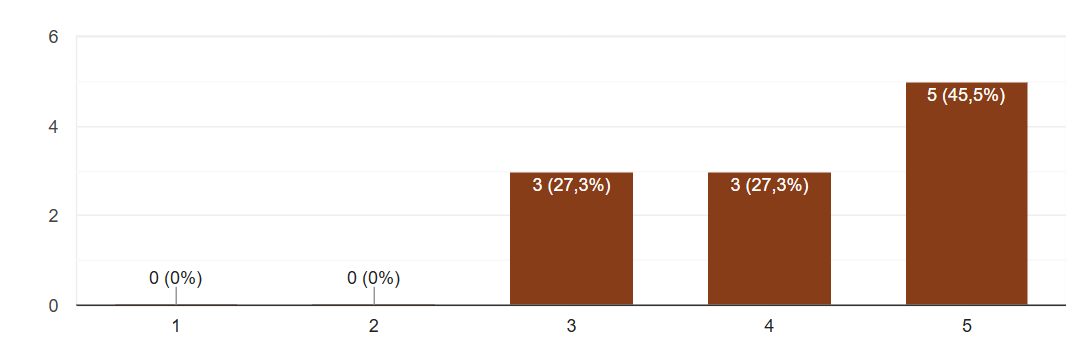
\includegraphics[width=1\linewidth]{bieu-do/chat-luong-do-hoa-tong-quan.png}
    \end{figure}
\end{frame}

% 5
\begin{frame}
    \frametitle{Chất lượng của các thẻ bài, item liên quan đến board game:}
    \begin{figure}[H]
        \centering
        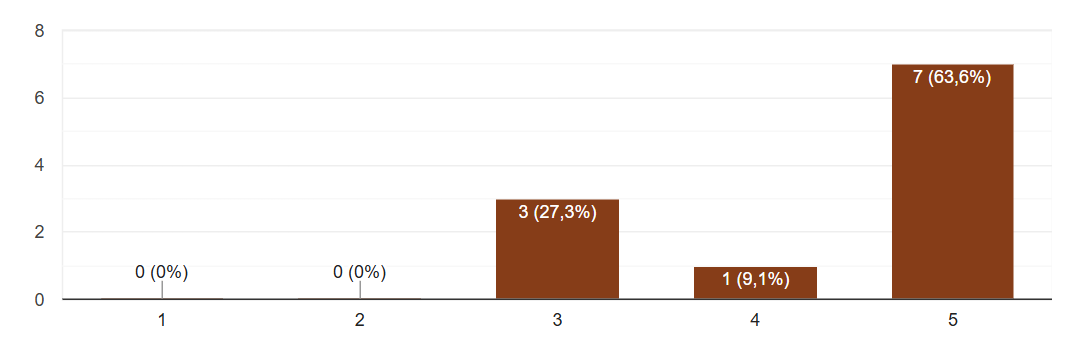
\includegraphics[width=1\linewidth]{bieu-do/the-bai-chat-luong.png}
    \end{figure}
\end{frame}


% 6
\begin{frame}
    \frametitle{Giao diện người dùng (UI) phù hợp:}
    \begin{figure}[H]
        \centering
        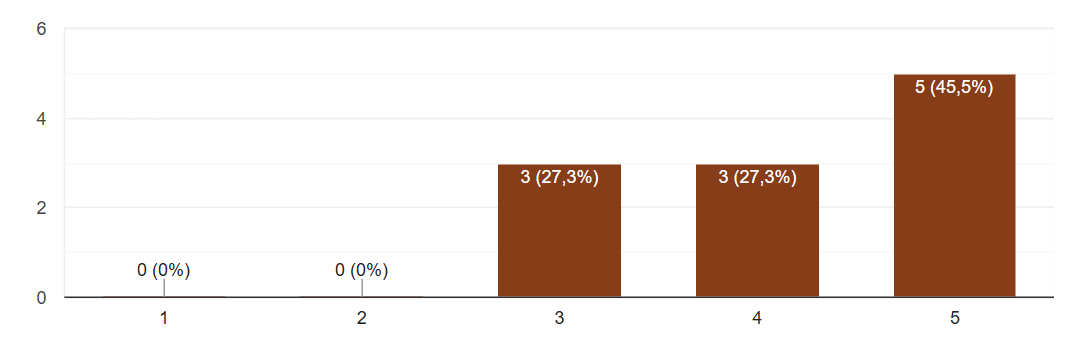
\includegraphics[width=1\linewidth]{bieu-do/ui-phu-hop.png}
    \end{figure}
\end{frame}

% 7
\begin{frame}
    \frametitle{Hiệu ứng âm thanh và nhạc nền phù hợp:}
    \begin{figure}[H]
        \centering
        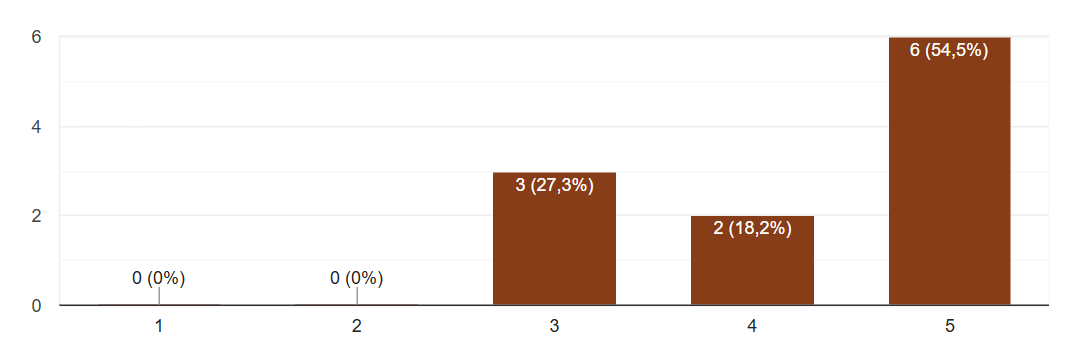
\includegraphics[width=1\linewidth]{bieu-do/am-thanh.png}
    \end{figure}
\end{frame}

% 15
\begin{frame}
    \frametitle{Lối chơi, độ hấp dẫn của board game - classic mode:}
    \begin{figure}[H]
        \centering
        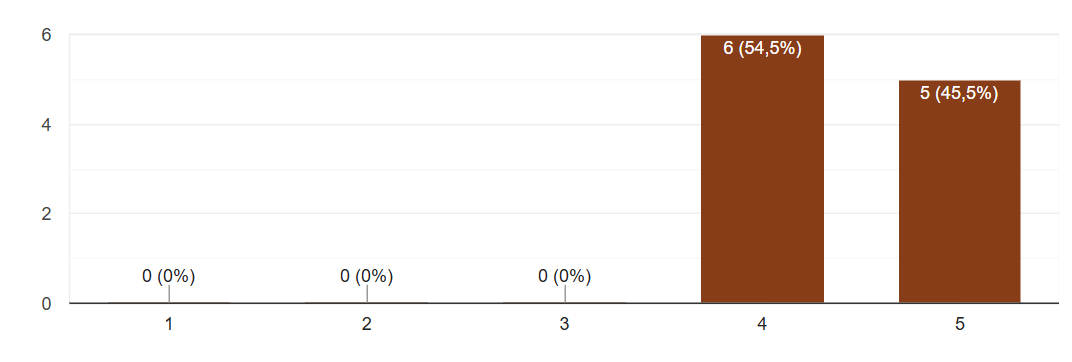
\includegraphics[width=1\linewidth]{bieu-do/classic-hap-dan.png}
    \end{figure}
\end{frame}

% 16
\begin{frame}
    \frametitle{Lối chơi, độ hấp dẫn của board game - day \& night mode:}
    \begin{figure}[H]
        \centering
        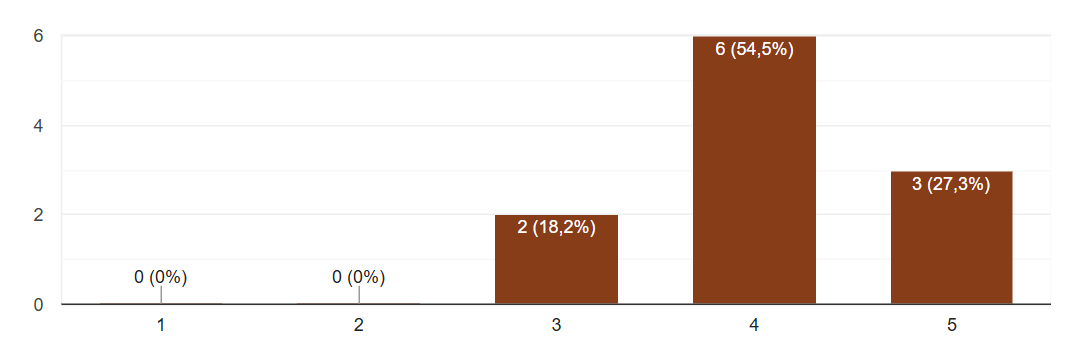
\includegraphics[width=1\linewidth]{bieu-do/day-nigh-hap-dan.png}
    \end{figure}
\end{frame}

% Slide 19: Hạn chế
\begin{frame}
\frametitle{Hạn chế}

\begin{columns}
    \column{0.5\textwidth}
    \begin{itemize}
        \item Số lượng map còn ít
        \item Chưa tối ưu hoàn toàn real-time networking
        \item Vẫn sử dụng mô hình Client-Host
    \end{itemize}
    
    \column{0.5\textwidth}
    \begin{itemize}
        \item Hiệu năng phụ thuộc vào Host
        \item Chưa kiểm thử với nhiều người chơi
        \item Thiếu một số tính năng nâng cao
    \end{itemize}
\end{columns}

\end{frame}


% SLIDE 20: Kế Hoạch Tiếp Theo
\begin{frame}
\frametitle{Kế hoạch tương lai}

\begin{columns}
    \column{0.5\textwidth}
    \begin{itemize}
        \item Mở rộng số lượng map và chế độ chơi
        \item Tối ưu hệ thống real-time networking
        \item Chuyển sang mô hình Client-Server
    \end{itemize}
    
    \column{0.5\textwidth}
    \begin{itemize}
        \item Bổ sung ranking và lưu dữ liệu server
        \item Thêm reconnect và anti-cheat
        \item Kiểm thử với số lượng người chơi lớn
    \end{itemize}
\end{columns}

\end{frame}